\begin{theorem}[теорема единственности]
	Пусть выполнены следующие условия:
	\begin{enumerate}
		\item Функция $f$ регулярна на области $G \subset \Cm$
		\item Множество $E \subset G$ "--- такое, что $f \equiv 0$ на $E$
		\item $E$ имеет предельную точку $z_0 \in G$
	\end{enumerate}
	
	Тогда $f \equiv 0$ на $G$.
\end{theorem}

\begin{proof}
	Из условия, существует последовательность попарно различных точек $\{z_n\} \subset E$ такая, что $\lim\limits_{n \to \infty}z_n = z_0$. Но $\forall n \in \N \cup \{0\}: f(z_n) = 0$, тогда, в силу непрерывности функции $f$, выполнено $f(z_0) = 0$. Кроме того, нуль $z_0$ "--- не изолированный. Значит, так как функция $f$ регулярна в $G$, то она представима в виде ряда Тейлора с центром в $z_0$: \(f(z) = \sum\limits_{n=0}^{\infty} c_n (z-z_0)^n\). Предположим, что функция не равна тождественному $0$ в какой-то окрестности $z_0$, тогда в её ряде Тейлора есть ненулевые члены. Выберем первый ненулевой член (пусть у него номер $m$) и вынесем его: \(f(z) = (z-z_0)^m \sum\limits_{n=0}^\infty c_{n+m}(z-z_0)^n:=(z-z_0)^m S(z), \: S(z_0)=c_m \Rightarrow\) из непрерывности $S(z)$ заключаем, что существует \(\mathring{B}_\varepsilon(z_0)\), такая, что на ней $S(z) \neq 0$. Так как \(\forall z \neq z_0\left(z-z_0 \neq 0 \right)\), есть проколотая окретсность \(z_0\), что в ней \(f\) нигде не ноль. А так как \(z_0\) --- предельная точка \(E\), то в любой её окрестности есть точки из \(E\), на которых она должна быть равна нулю. Противоречие. Значит $f \equiv 0$ на наибольшем круге $K \subset G$ с центром в точке $z_0$.
	
	Проверим теперь, что $\forall z_1 \in G \bs K : f(z_1) = 0$. Пусть это не так, и для некоторой точки $z_1 \in G \bs K$ выполнено $f(z_1) \ne 0$, тогда, из регулярности, на некотором круге $K_1 \subset G$ с центром в точке $z_1$ выполнено $f \ne 0$. Поскольку множество $G$ связно, существует лежащая в $G$ кривая $\gamma$ с параметризацией $z = \sigma(t)$, $t \in [a, b]$, соединяющая точки $z_0$ и $z_1, \sigma(a) = z_0$ и \(\sigma(b)=z_1\). Положим $$\tau := \inf\{t \in [a, b]: f(\sigma(t)) \ne 0\},\;\; z^* := \sigma(\tau).$$ Тогда:
	\begin{center}
		\scalebox{1.1}{
			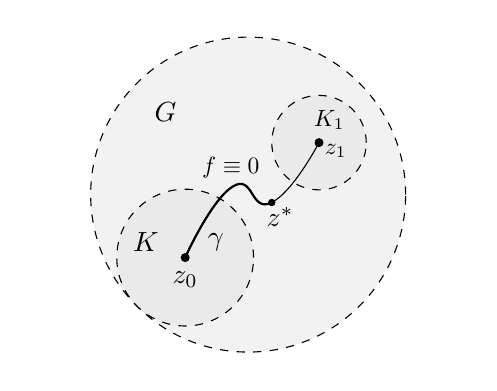
\begin{tikzpicture}
				\clip (-2.8, -2.14) rectangle (2.8, 2.12);
				
				\fill [opacity=0.05] (0,0) circle [radius=2];
				\draw[black, dashed] (0,0) circle[radius=2];
				
				\node[] at (-1.05, 1.05) {$G$};
				
				\fill [opacity=0.03] (0,0) (-0.8, -0.8) circle[radius=2 - 0.8 * 1.414];
				\draw[black,dashed] (-0.8, -0.8) circle[radius=2 - 0.8 * 1.41421];
				\node[] at (-1.3, -0.6) {$K$};
				\node[draw, circle, inner sep=1pt, fill, black, label=below:$z_0$] at (-0.8, -0.8) {};
				
				\node[] at (-0.41, -0.6) {$\gamma$};
				
				\fill [opacity=0.03] (0,0) (0.9, 0.66) circle[radius=0.6];
				\draw[black,dashed] (0.9, 0.66) circle[radius=0.6];
				\node[] at (1.03, 0.95) {\scalebox{0.85}{$K_1$}};
				\node[draw, circle, inner sep=1pt, fill, black, label={right, shift={(-3pt,-3pt)}:\scalebox{0.85}{$z_1$}}] at (0.9, 0.66) {};
				
				\path
				coordinate (start) at (-0.8, -0.8)
				coordinate (endd) at (0.9, 0.66);
				
				\begin{scope}
					\clip(-3, -2.5) rectangle (0.3, 1);
					\draw[style={thick}] plot [smooth, tension=0.9] coordinates {(start) (-0.2, 0.1) (0.3, -0.1) (endd)};
				\end{scope}
				
				\draw[] plot [smooth, tension=0.9] coordinates {(start) (-0.2, 0.1) (0.3, -0.1) (endd)};
				\node[draw, circle, inner sep=0.8pt, fill, black, label={below, shift={(3pt,3pt)}:$z^*$}] at (0.3, -0.1) {};
				\node[] at (-0.22, 0.34) {\scalebox{0.85}{$f \equiv 0$}};
			\end{tikzpicture}
		}
	\end{center}
	
	По предположению, $\tau \in (a, b)$ и, в силу непрерывности, $f(z^*) = 0$, причем нуль $z^*$ не является изолированным. Тогда повторим рассуждения из начала теоремы и получим, что существует окрестность точки \(\tau\), в которой \(f\) тождественно 0, а это противоречит выбору \(\tau\).
\end{proof}

\begin{corollary}
	Пусть выполнены следующие условия:
	\begin{enumerate}
		\item Функции $g, h$ регулярны на области $G \subset \Cm$
		\item Множество $E \subset G$ "--- такое, что $g \equiv h$ на $E$
		\item $E$ имеет предельную точку $z_0 \in G$
	\end{enumerate}
	
	Тогда $g \equiv h$ на $G$.
\end{corollary}

\begin{proof}
	Применим теорему единственности к функции $g - h$.
\end{proof}

\begin{unnecessary}
    \begin{note}
    	Из теоремы единственности также следует, что тот способ, которым мы доопределили экспоненту на $\Cm$, "--- единственный, при котором полученное продолжение является регулярным.
    \end{note}

    \begin{example}
    	Рассмотрим следующее дифференциальное уравнение:
    	\[y^{(n)} + a_1y^{(n-1)} + \dotsb + a_ny = 0\]
    	
    	Пусть $\widetilde y$ "--- некоторое частное решение уравнения. Тогда из теории дифференциальных уравнений мы знаем, какой вид имеет $\widetilde y$, и можем утверждать, что ее продолжение на $\Cm$ регулярно. Применяя теорему единственности к функции $g := \widetilde y^{(n)} + a_1\widetilde y^{(n-1)} + \dotsb + a_n\widetilde y$, получим, что $g \equiv 0$ не только на $\R$, но и на $\Cm$.
    \end{example}
\end{unnecessary}